%%%%%%%% ICML 2024 EXAMPLE LATEX SUBMISSION FILE %%%%%%%%%%%%%%%%%

\documentclass{article}

% Recommended, but optional, packages for figures and better typesetting:
\usepackage{microtype}
\usepackage{graphicx}
\usepackage{subfigure}
\usepackage{booktabs} % for professional tables

% hyperref makes hyperlinks in the resulting PDF.
% If your build breaks (sometimes temporarily if a hyperlink spans a page)
% please comment out the following usepackage line and replace
% \usepackage{icml2019} with \usepackage[nohyperref]{icml2019} above.
\usepackage{hyperref}

% Attempt to make hyperref and algorithmic work together better:
\newcommand{\theHalgorithm}{\arabic{algorithm}}

% Use the following line for the initial blind version submitted for review:
%\usepackage{icml2024}

% If accepted, instead use the following line for the camera-ready submission:
\usepackage[accepted]{icml2024}
\icmltitlerunning{COSE474-2024F: Final Project}

\begin{document}

\twocolumn[
\icmltitle{Monocular Depth Estimation with Segment Anything Model}

% It is OKAY to include author information, even for blind
% submissions: the style file will automatically remove it for you
% unless you've provided the [accepted] option to the icml2019
% package.

% List of affiliations: The first argument should be a (short)
% identifier you will use later to specify author affiliations
% Academic affiliations should list Department, University, City, Region, Country
% Industry affiliations should list Company, City, Region, Country

% You can specify symbols, otherwise they are numbered in order.
% Ideally, you should not use this facility. Affiliations will be numbered
% in order of appearance and this is the preferred way.
\icmlsetsymbol{equal}{*}

\begin{icmlauthorlist}
\icmlauthor{Sanghwa Song}{}
\end{icmlauthorlist}

%\icmlaffiliation{ku}{Department of Computer Science \& Engineering, Korea University, Seoul, Korea}

%\icmlcorrespondingauthor{the}{myemail@korea.ac.kr}
%\icmlcorrespondingauthor{Eee Pppp}{ep@eden.co.uk}

% You may provide any keywords that you
% find helpful for describing your paper; these are used to populate
% the "keywords" metadata in the PDF but will not be shown in the document
\icmlkeywords{Machine Learning, ICML}

\vskip 0.3in
]

% this must go after the closing bracket ] following \twocolumn[ ...

\section{Introduction}

\subsection{Motivation}

Monocular depth estimation is a crucial task in computer vision with applications in various fields such as autonomous driving, robotics, and augmented reality. But recovering 3D information from single image remains challenging due to data ambiguity and model limitations.

The Segment Anything Model (SAM) \cite{SAM} demonstrates strong object segmentation capabilities, and we hypothesize its encoder can provide valuable features for depth estimation by associating similar depths within objects and distinguishing discontinuities at boundaries. This study explores the potential of utilizing the pre-trained encoder from SAM for monocular depth estimation.

By investigating its applicability in this context, we aim to assess whether SAM's capabilities can effectively address the existing challenges in depth estimation and pave the way for more efficient and precise 3D scene understanding. In conclusion, we suggest that while SAM provides a strong foundation, its application to depth estimation tasks requires careful consideration and further adaptations to overcome its inherent limitations.

\subsection{Problem definition}

An image can contain one or more objects and can have several information about the objects. One of them is information about the depth, and our goal is to predict the depth from a single RGB image.

Given a single RGB image $ I \in R^{ H \times W \times 3 } $, the task is to estimate a depth map $ D \in R^{ H \times W } $. Our goal is to find a function $ f: I \rightarrow D $ that maps input image to depth map.

\begin{figure}[ht]
\centering
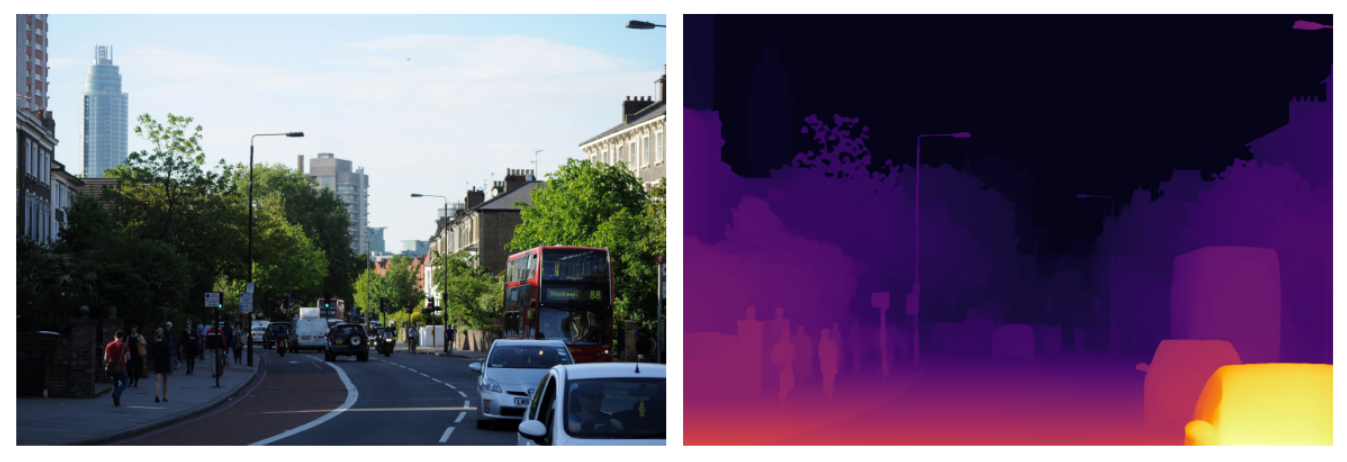
\includegraphics[width=0.5\textwidth]{monocular-depth-estimation.png}
\label{fig:model-comparison}
\end{figure}

\section{Methods}

\subsection{Model architecture}

The given image is encoded using SAM encoder to generate a feature map. Specifically, we utilize SlimSAM \cite{SlimSAM}, a variant of SAM, to enable faster computation. The feature map is then decoded into a depth map through residual connections and transposed convolutions. The output depth map is resized to match the target size using bilinear interpolation. Finally, a loss function is applied to compare the predictions with the ground truth. Mean Squared Error (MSE) is used as a loss function for simplicity.

\begin{figure}[ht]
\centering
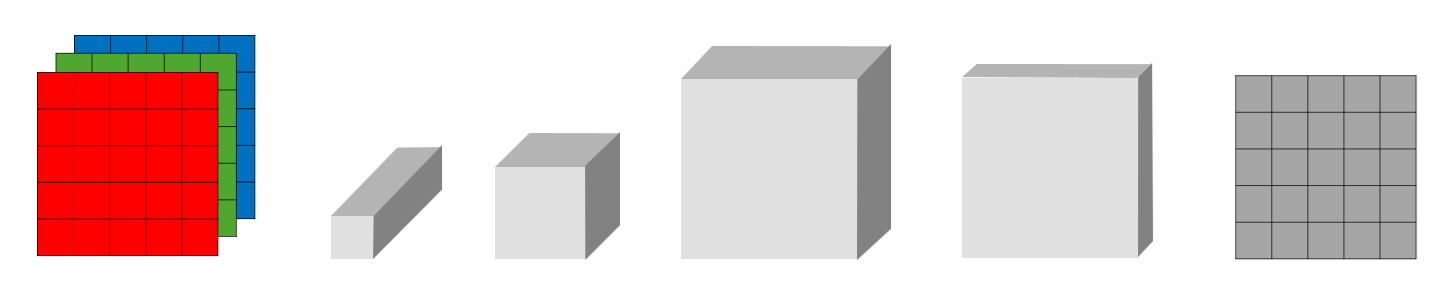
\includegraphics[width=0.45\textwidth]{model-figure.png}
\caption{Model Architecture}
\label{fig:model-architecture}
\end{figure}

\begin{algorithm}[]
\caption{Depth Estimation Using SAM Encoder and CNN Decoder}

\begin{algorithmic}[1]
\REQUIRE Input image $I$ of size $H \times W \times 3$
\ENSURE Estimated depth map $\hat{D}$ of size $H \times W$.

\STATE \textbf{Encode the input image.}\\
Input the image $I$ into the SAM encoder.\\
Obtain the feature map $F$ of size $256 \times 64 \times 64$.\\

\STATE \textbf{Decode the feature map.}\\
Pass $F$ through the decoder, utilizing residual connections and transposed convolution.\\
Obtain the decoded depth map $\tilde{D}$ of size $256 \times 256$.\\

\STATE \textbf{Resize the output feature.}\\
Resize the target depth map $\tilde{D}$ to $\hat{D}$ of size $H \times W$ using bilinear interpolation.\\

\STATE \textbf{Compute the loss.}\\
Apply the Mean Squared Error (MSE) loss function between $\hat{D}$ and the target depth map $D$:\\

\[
\mathcal{L}_{\text{MSE}} = \frac{1}{n} \sum_{i=1}^n (\hat{D}_i - D_i)^2
\]

\STATE \textbf{Backpropagate and update.}\\
Use the computed loss $\mathcal{L}_{\text{MSE}}$ to backpropagate through the network and update the model parameters.\\

\end{algorithmic}
\end{algorithm}

\section{Experiments}

\subsection{Dataset}

We use \href{https://cs.nyu.edu/~fergus/datasets/nyu_depth_v2.html}{NYU Depth Dataset V2} \cite{NYU-Depth-V2-Dataset}. NYU Depth Dataset V2 is a widely-used dataset for research in 3D computer vision, particularly focusing on tasks like depth estimation and indoor scene understanding. It provides paired RGB images and depth maps collected using a Microsoft Kinect sensor in indoor environments.

Data augmentation techniques such as random cropping and flipping are also applied. The dataset is split into 90\% for training, 9\% for validation, and 1\% for testing.

\begin{figure}[ht]
\centering
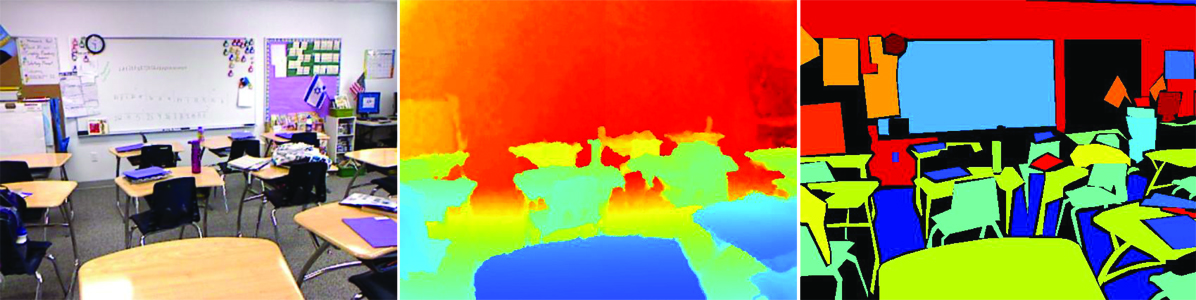
\includegraphics[width=0.5\textwidth]{nyu-depth-v2.jpg}
\label{fig:nyu-depth-v2}
\end{figure}

\subsection{Experimental design}

The model is trained using the Adam optimizer with a learning rate of 0.001 and a batch size of 4 for 1 epochs. The parameters of the pre-trained SAM backbone are frozen during training. The Mean Squared Error (MSE) is used as a loss function. Experiments are conducted on an NVIDIA L4 GPU in Colab Pro with PyTorch. The training was restricted to a single epoch due to limited GPU resources. 

\subsection{Results}

To evaluate the performance of our depth estimation model, we use Depth-Anything-V2-Small as our baseline for comparison, which is one of the state-of-the-art models. We use Absolute Relative Error (Abs Rel) and Root Mean Squared Error (RMSE) as evaluation metrics. Abs Rel ensures fair evaluation across depths with its scale-invariant property, while RMSE highlights significant deviations by penalizing larger errors.

{\small

\begin{equation}
    \textnormal{Abs Rel} = \frac{1}{N} \sum_{i=1}^{N} \frac{|D_i - \hat{D}_i|}{D_i}
\end{equation}

\begin{equation}
    \textnormal{RMSE} = \sqrt{\frac{1}{N} \sum_{i=1}^{N} (D_i - \hat{D}_i)^2}
\end{equation}

}

\begin{table}[ht]
\centering
\caption{Comparison of the model performance}
\label{tab:quantitative-results}
\begin{tabular}{|l|c|c|}
\hline
\textbf{Model}                 & \textbf{Abs Rel} & \textbf{RMSE} \\ \hline
Depth-Anything-V2-small        & \textbf{0.253}                      & \textbf{0.107}                         \\ \hline
Ours                  & 0.463             & 0.131                \\ \hline
\end{tabular}
\end{table}

Next, we present qualitative comparisons of depth estimation results. Each figure consists of input RGB images, predicted depth maps from our method, predictions from Depth-Anything-V2-Small, and the corresponding ground truth depth maps.

\begin{figure}[ht]
\centering
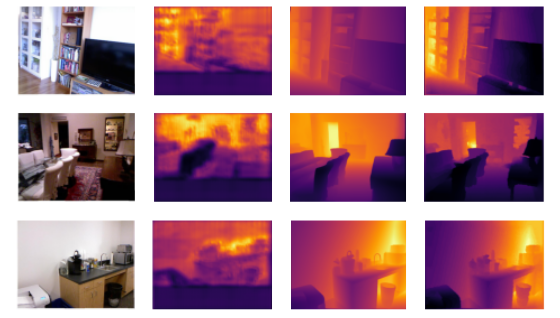
\includegraphics[width=0.5\textwidth]{model-comparison.png}
\caption{Model Comparison}
\label{fig:model-comparison}
\end{figure}

\section{Discussion}

\subsection{Analysis}

Our method showed inferior results compared to Depth-Anything-V2-Small in both quantitative and qualitative results. 

Our analysis indicates that the Segment Anything model, used as a pre-trained backbone, demonstrates a tendency to predict different depths for different objects. This behavior is likely reflects the intuition that spatial similarity implies similar depth. While this approach is effective to capture spatial relationships, it also has a limitation: Different adjacent objects with similar depths may not be correctly modeled. For example, the first image in Figure 2 \ref{fig:model-comparison}, the pre-trained model tends to overemphasize object differentiation, leading to incorrect depth predictions.

Another issue observed in the predicted depth maps is their uneven and bumpy appearance, particularly in regions that are expected to exhibit smooth depth transitions. It is likely influenced by the simplicity of the loss function used during training. The Mean Squared Error (MSE) loss, while effective for minimizing pixel-wise differences between predictions and ground truth, does not explicitly enforce spatial smoothness or continuity in the depth map. As a result, the model may struggle to capture globally consistent depth information, leading to localized irregularities.

Main reason for the low performance of our approach is the significant computational cost involved, which exceeded our available resources. This limitation restricted the model's training process, resulting in unsatisfactory depth predictions.

\subsection{Future direction}

Our findings indicate that SAM, while effective for segmentation tasks, may not be inherently optimized for depth estimation. Future work should focus on identifying and leveraging pre-trained models specifically designed or fine-tuned for depth estimation. This direction could provide more suitable feature representations, leading to improved depth predictions.

An important area for improvement is the design of the loss function. While the Mean Squared Error (MSE) loss is simple and efficient, it does not account for spatial continuity or structural consistency in the depth maps, likely contributing to the uneven predictions observed. Future work should explore more advanced loss functions that promote smoothness and structural alignment in depth predictions.

The computational cost of using SAM as a backbone was a significant limitation in this study. To overcome this, future efforts should focus on acquiring sufficient computational resources or employing resource-efficient techniques. And we should aim to train models on a broader range of datasets to improve the model's generalization capabilities. It can help the model adapt to different depth characteristics across diverse environments. 

\section{Conclusion}

In this study, we explored the potential of using the Segment Anything Model (SAM) as a backbone for monocular depth estimation. While SAM demonstrates strong capabilities in object segmentation, our findings indicate that its application to depth estimation tasks faces notable challenges. 

The limitations of our approach arise from SAM's segmentation-focused nature, which overemphasizes object boundaries and disrupts depth continuity. Additionally, the simplicity of Mean Squared Error (MSE) loss led to uneven depth predictions, lacking spatial smoothness and consistency. Limited computational resources further constrained the training process, affecting the model's lower performance.

Despite these challenges, this work highlights the potential of leveraging pre-trained models for depth estimation tasks. Future research should focus on exploring pre-trained models optimized for depth-related tasks with depth-specific loss functions and addressing computational constraints when using pre-trained models.

\bibliography{main}
\bibliographystyle{icml2024}
\clearpage

\end{document}
